\chapter{Infectome pipeline}

\section{Human microbiome in cell-free DNA}

The human microbiome is now recognized as an important contributor to human health \cite{Consortium:2012bb}. NGS applied to external body sites have been very fruitful, as these sites can be easily sampled in large cohort studies in order to assemble populate-wide statistics on microbial composition. Yet, little is known about the microbial composition of deeper tissues, as it is challenging to access them.
  
Parallel efforts have focused using NGS as a tool to assay blood. These efforts take advantage of a phenomenon first described in 1947 by Mandel and Metais \cite{Quake:2012iy}. They discovered that blood contains circulating cell-free DNA. These DNA fragments enter blood as the detritus of dead and apoptosed cells, and are likely nucleosome-protected fragments enriched in circulation. Methods of molecular counting, notably NGS, have taken advantage of this phenomenon, using a new era of universal noninvasive diagnostic tests. Starting with detection of aneuploidies (such as Down syndrome) for pregnant women  \cite{Fan:2008ww}, molecular coating by NGS has been extended to organ transplants \cite{DeVlaminck:2013hl} (which can be thought of as genome transplants) and cancers \cite{Newman:2014ik}. The in the latter two cases, specific mutations can be used to resolve donor- or cancer-derived DNA fragments in circulation.

DNA species may correlate with health, their greatest value has been to measure the pro- portion of foreign genomes within an individual. Cancer-related mutations can be used to some extent to determine the progress of disease (2 ), male chromosomal markers can be used for prenatal sex determination (3 ), and, in a sim- ilar fashion, women who have received organ transplants from males can be monitored for the amount of organ- specific DNA.

In a recent study, it was shown that non-human (microbial, fungal, and viral) derived cell-free DNA fragments can purified from blood and counted using NGS \cite{DeVlaminck:2013hl}. While translocation of microorganisms, or microorganism components, from the lumen of the GI tract into the systemic circulation can occur, it often has detrimental consequences, including activation of the immune system, and in extreme cases it can lead to septic shock \cite{Brenchley:2012bm}. The absence of acute sepsis of similar symptoms in our cohort further suggests that the majority of detected organisms are innocuous detritus of dead cells. Nevertheless, their existence suggests that microorganism-derived cell-free DNA fragments in blood can serve as a snapshot of microbial composition  in diverse body sites and / or provide a way to monitor infections.

\section{Pipeline for capturing microbiome in cell-free DNA}

The general strategy for read assignment for any clinical sampled has been well-described. Computational subtraction of reads corresponding to the host (e.g., human) is typically performed using short-read aligners (e.g, Bowtie) and is followed by alignment (e.g., BLAST) to reference databases that contain sequences from candidate pathogens (e.g., NCBI). Yet, four challenges frustrate the use of NGS for infectious disease detection in cell-free DNA. Published strategies for detection of microorganism derived cell-free DNA follows this general workflow \cite{DeVlaminck:2013hl} though also employs an algorithm to reduce ambiguity in these alignments \cite{Xia:2011it}. In spite of this, four challenges underlie this analysis.

\textbf{Large data} Alignment and classification algorithms must contend with massive amounts of sequence data. Recent advances in NGS technologies have resulted in instruments that are capable of producing >100 gigabases (Gb) of reads in a day. Furthermore, reference databases of host and pathogen sequences used by BLAST range in size from 2 Gb for viruses to 3.1 Gb for the human genome to 42 Gb for all nucleotide sequences in the National Center for Biotechnology Information (NCBI) nucleotide (nt) collection (as of January 2013). 

\begin{figure*}
\center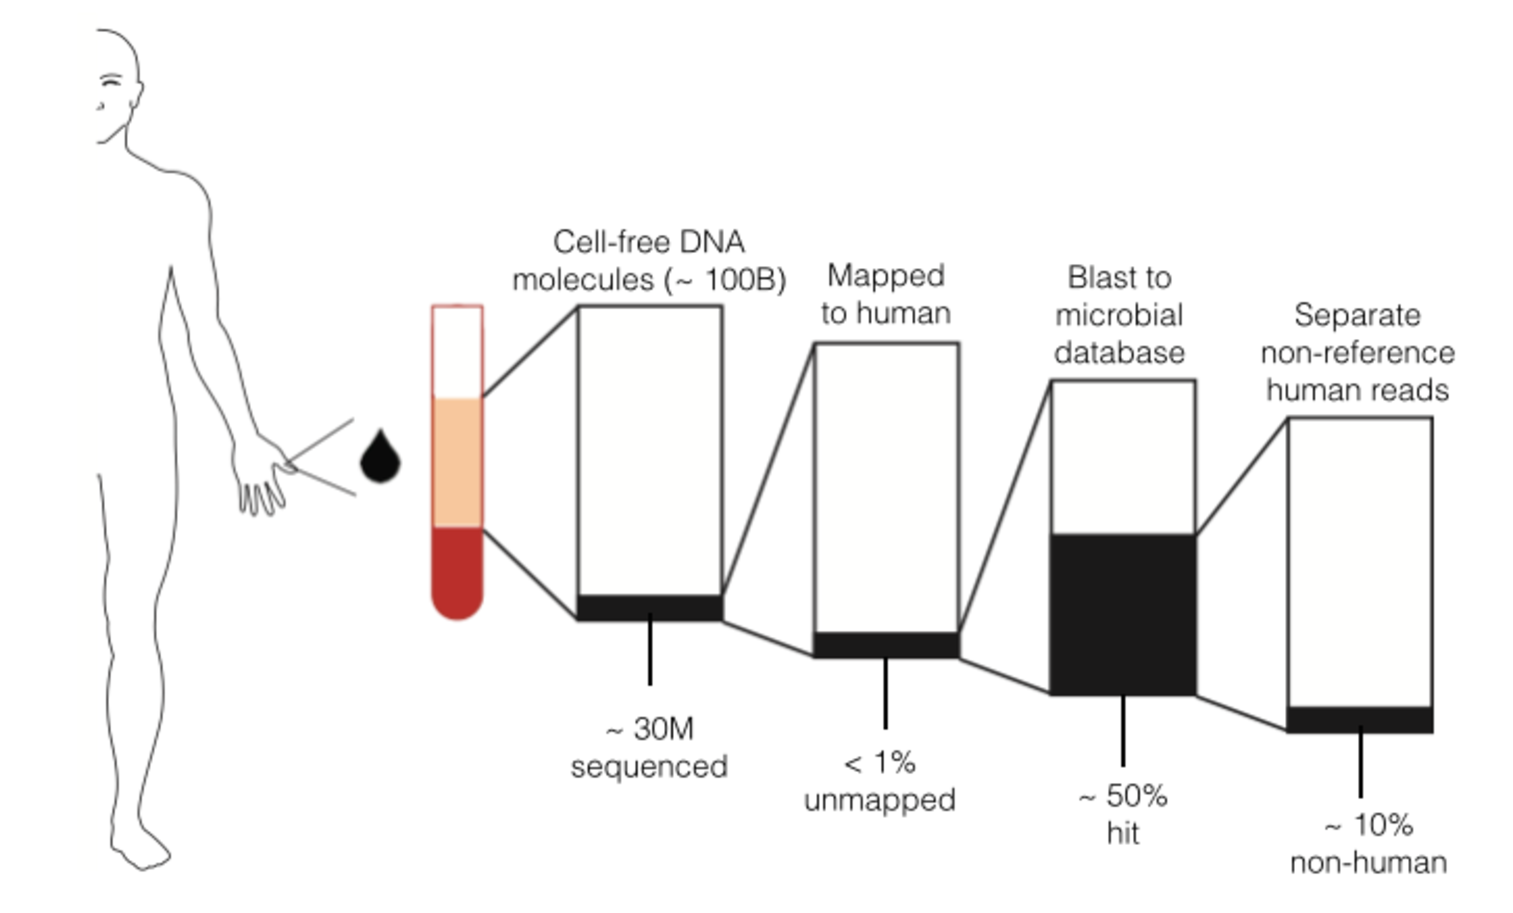
\includegraphics[width=100mm,scale=0.5]{Figures/Fig3}
\caption{Isolation of non-human cell-free DNA.}
\label{fig:Fig3}
\end{figure*}

\textbf{Signal} Only a small fraction of short NGS reads in clinical metagenomic data typically correspond to pathogens. This is particularly true in the case of cell-free DNA, as non-human cell-free DNA is < 1\% of mapped reads. Furthermore, only a fraction of these un-mapped reads are actually derived from non-human sources, as most is either human DNA that is not found in the reference index used for mapping or does not align to the BLAST database used after mapping (Figure ~\ref{fig:Fig3}). 

\textbf{Speed} BLAST is likely too slow for routine clinical analysis of NGS metagenomics data, as end-to-end processing times, even on multicore computational servers, can take several days to weeks.  Analysis pipelines that use faster, albeit less sensitive, algorithms upfront for host computational subtraction, such as PathSeq, still rely on traditional BLAST approaches for final pathogen determination.  

\textbf{Interpretation} the data must bed organized and presented at scale, across large clinical cohorts, such that it is intuitive for researchers and clinicians.

The signal problem will largely be addressed through bio-chemical methods to enrich for non-human derived nucleic acids. Furthermore, the speed problem has recently been addressed using faster alignment algorithms, such as SNAP in place of BLAST and RAPSearch for assignment of de novo contig assemblies in order to classify potentially novel organisms \cite{Naccache:2014gk}. Despite these technical advances, there will probably continue to be a gap between the availability of such data and the ability to comprehensively interpret the results for clinical decision making. With this in mind, our emphasis was to develop a full application stack that performed both processing and visualizations to aid interpretation of all microorganisms in cell-free DNA sequence data. 

In order to achieve this, we developed an application stack written in Python that used the Django web-development framework with the Matplotlib visualization library \cite{Hunter:2007ux} and the Pandas library for data analysis. We built the Django application on top of a Postgres database using Sqlalchemy. The first part of the pipeline work as described previously, using several algorithms to compute relative abundance of microorganisms in each sample \cite{DeVlaminck:2013hl}. Reference files (e.g., taxonomic table), output files (e.g., BLAST results), and sample -meta data then written to Postgres. The tables in Postgres are referenced directly by the Django application (Figure ~\ref{fig:Fig4}).

\begin{figure*}
\center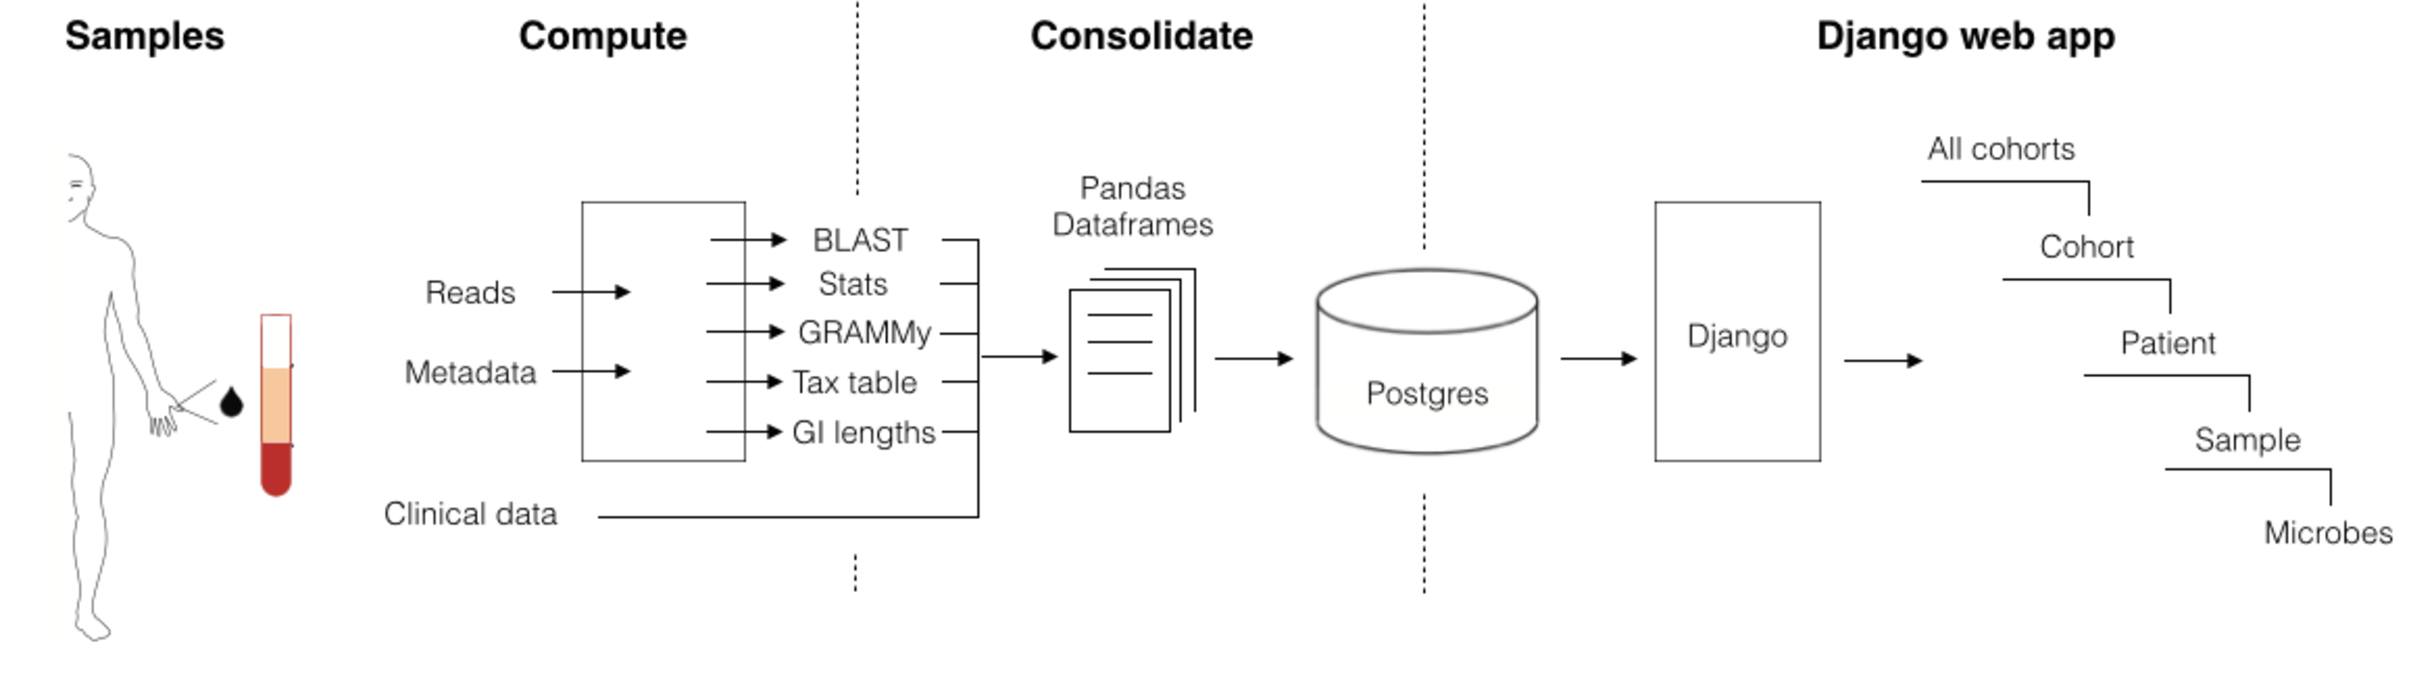
\includegraphics[width=150mm,scale=0.5]{Figures/Fig4}
\caption{Django application for infectome data.}
\label{fig:Fig4}
\end{figure*}

Browsers have been broadly useful after their emergence in the early 2000s in response to rapid improvements in sequencing and array-based platforms are resulting in a flood of diverse genome-wide data \cite{ODonoghue:2010bd}. In turn, our application was designed to be data browser that can be used to explore cell-free DNA infection (or \emph{Infectome}) data at all relevant scales. Indeed, we designed the application for intuitive navigation of this multi-scale data: each cohort is comprised of patients, which in turn may have many samples. In each sample, there may be thousands of unique infections identified in the cell-free DNA sequencing. Furthermore, infections may be viewed at different levels of taxonomic complexity, such as genus or species. 

With this in mind, we designed the Django application to present a series of web pages that reflect each relevant level of organization in the data. The cohort page reflects  the highest level of organization. It presents a table of patients, which is sorted by the number of samples per patient, that provides a link to explore data for each patient in the cohort. It also provides cohort-level histograms that explain both incidence of the identified infection (fraction of samples in which each identified infection is found) as well as the load per sample (the number of infections identified per sample). In addition, it provides a table of sorted infections by prevalence within the cohort. Finally, it provides a toggle that allows the data to be presented at different levels of taxonomic resolution, from genus to species (Figure ~\ref{fig:Fig5}). Collectively, this make is possible to navigate the data in two primary ways: it is possible to take a patient-centric approach to the data and examine data for specified patients. Or, it is possible to take an infection-centric approach to the data and examine simply the infections identified in the cohort across patients. 

\begin{figure*}
\center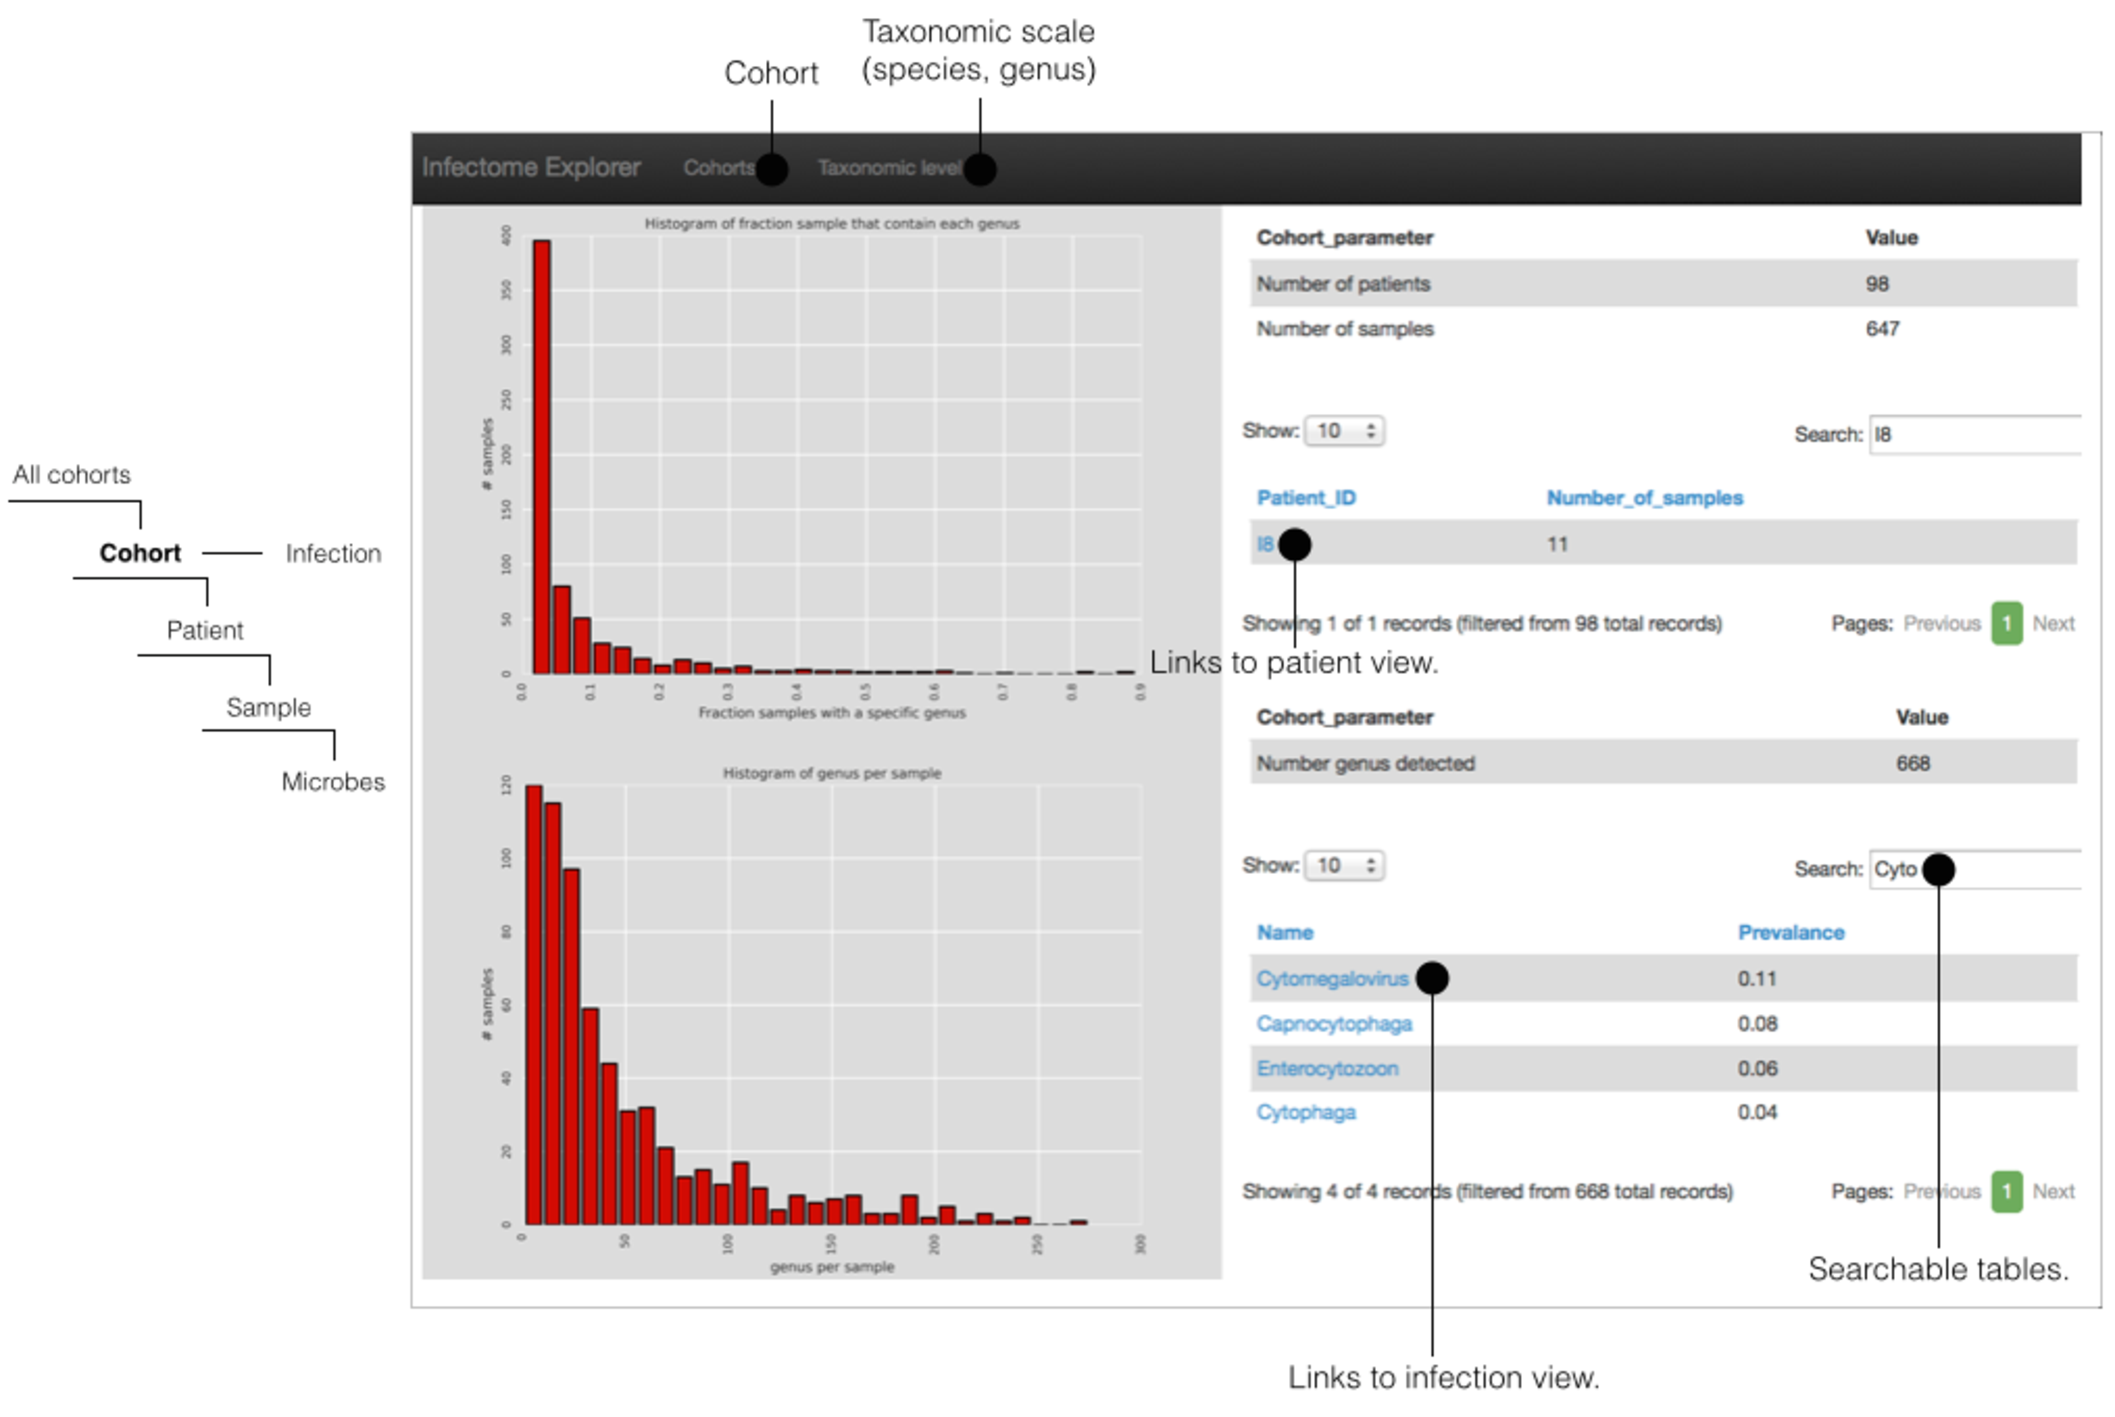
\includegraphics[width=150mm,scale=0.5]{Figures/Fig5}
\caption{Cohort data}
\label{fig:Fig5}
\end{figure*}

The patient-centric approach can be used to quickly identify the infections identified within a specified patient at a specified taxonomic scale (e.g., genus or species). In order to present this information intuitively, we transform the raw abundance measurements returned by the sequencing pipeline The pipeline uses an algorithm (GRAMMy) to process the raw BLAST results; GRAMMy addresses two problems. First, each organism has a different genome size and, in turn, genome size affects the number of reads expected for each. Second, reads often align to multiple genomes. Taking these into account, GRAMMy performs a maximum likelihood estimation for read assignment to each organism and provides relative abundance measurement per organism per sample. From this measurment, we back out an estimate for absolute read counts per genome. With this value, we compute a coverage ratio between each infection and human for that sample and scale this value by $10^6$ to get relative genome copies per million ($gcm$). In isolation, this value is not particularly intuitive: it indicates the number of genome copies for a given infection relative to human in that sample. For presentation, we simply compute a percentile (Figure ~\ref{fig:Fig6}) for each $gcm$ value with respect to the cohort for that infection. In turn, the percentile indicates the magnitude of each measurement relative to what is observed across the cohort. 

\begin{figure*}
\center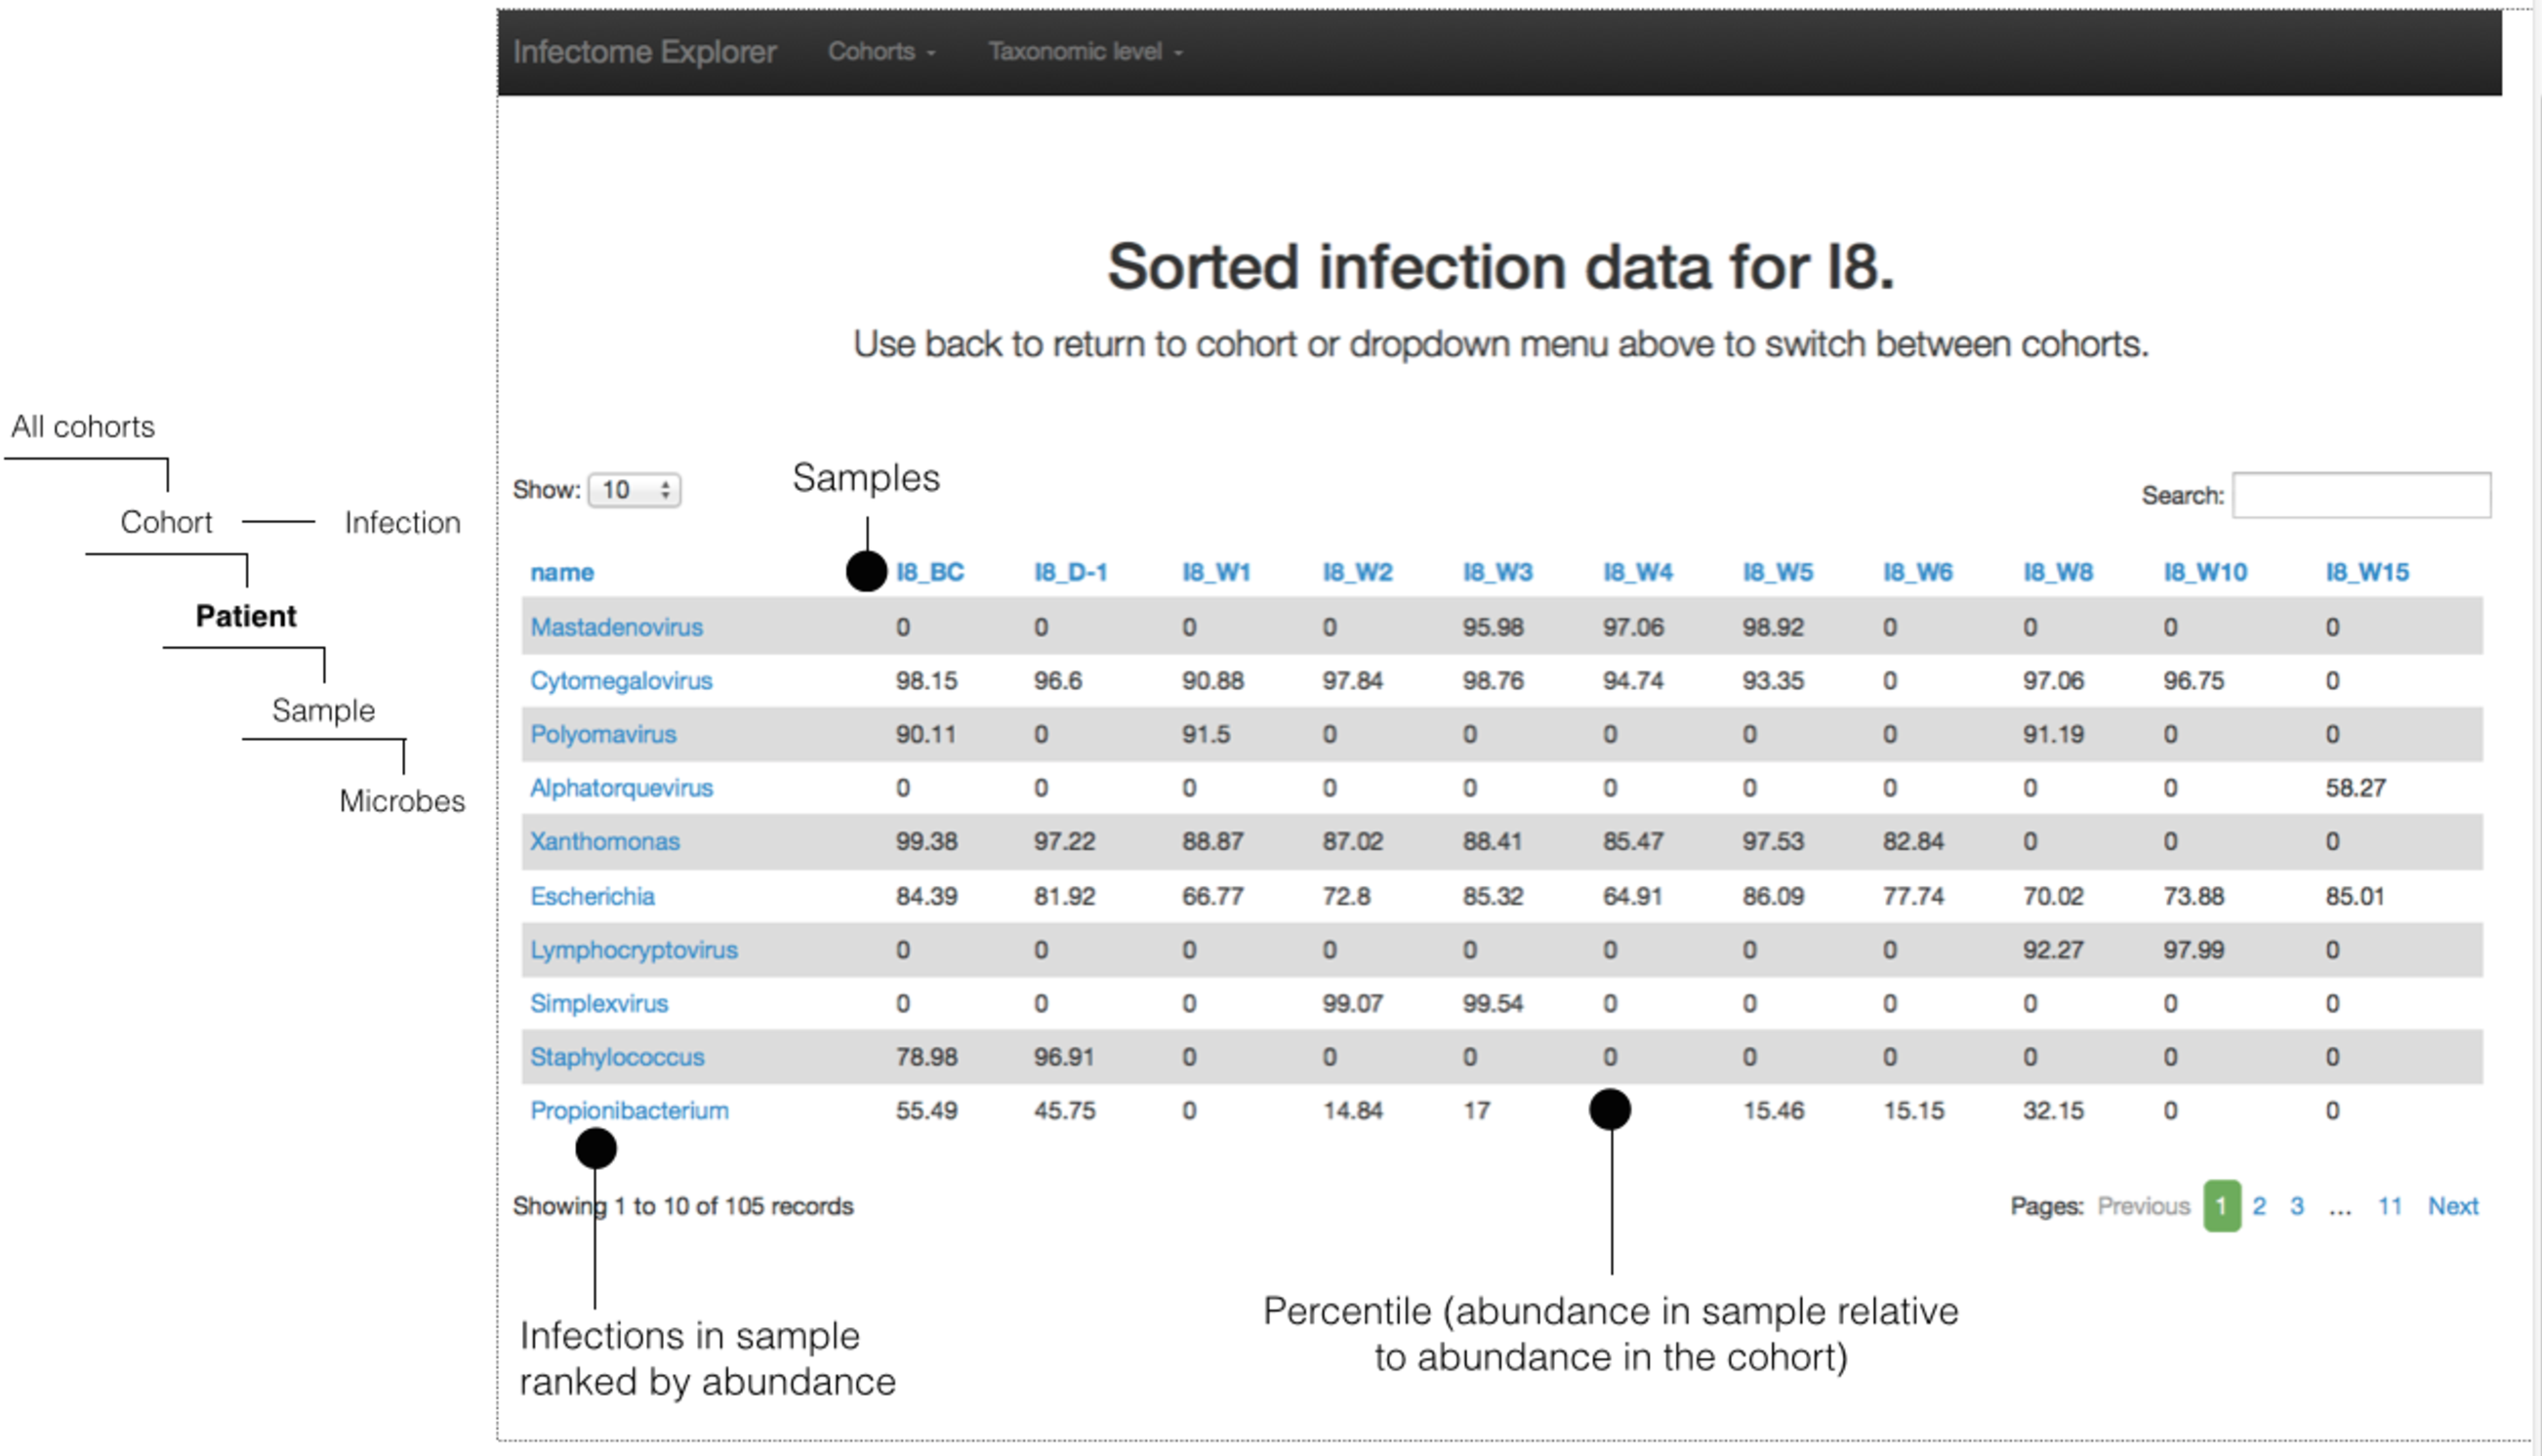
\includegraphics[width=150mm,scale=0.5]{Figures/Fig6}
\caption{Patient data}
\label{fig:Fig6}
\end{figure*}

From the patient view, it is possible to drill down into each identified infection. In this case, it is useful to know both the timeseries data for that infection as well as more detailed information about read coverage across the microbial genome. Both measurements can provide greater confidence about the legitimacy of a given signal. For example, a consistent infection timeseries across samples supports likelihood of a bona-fire infection relative to a spurious signal found in one sample or a higher irregular pattern. Furthermore, coverage is computed simply by aggregating GIs (individual sequence records in the BLAST database) for each taxID, lining the GIs up continuously into a composite "genome", and then evaluating reads with respect to position across this composite genome. Irregular coverage patters may be indicative of 
database contamination whereas consistent patters across the composite genome support presence of the identified infection. Using data from a bone marrow transplant cohort, we show both timeseries and coverage data collected for a particular patient (I8), Figure ~\ref{fig:Fig7}).

\begin{figure*}
\center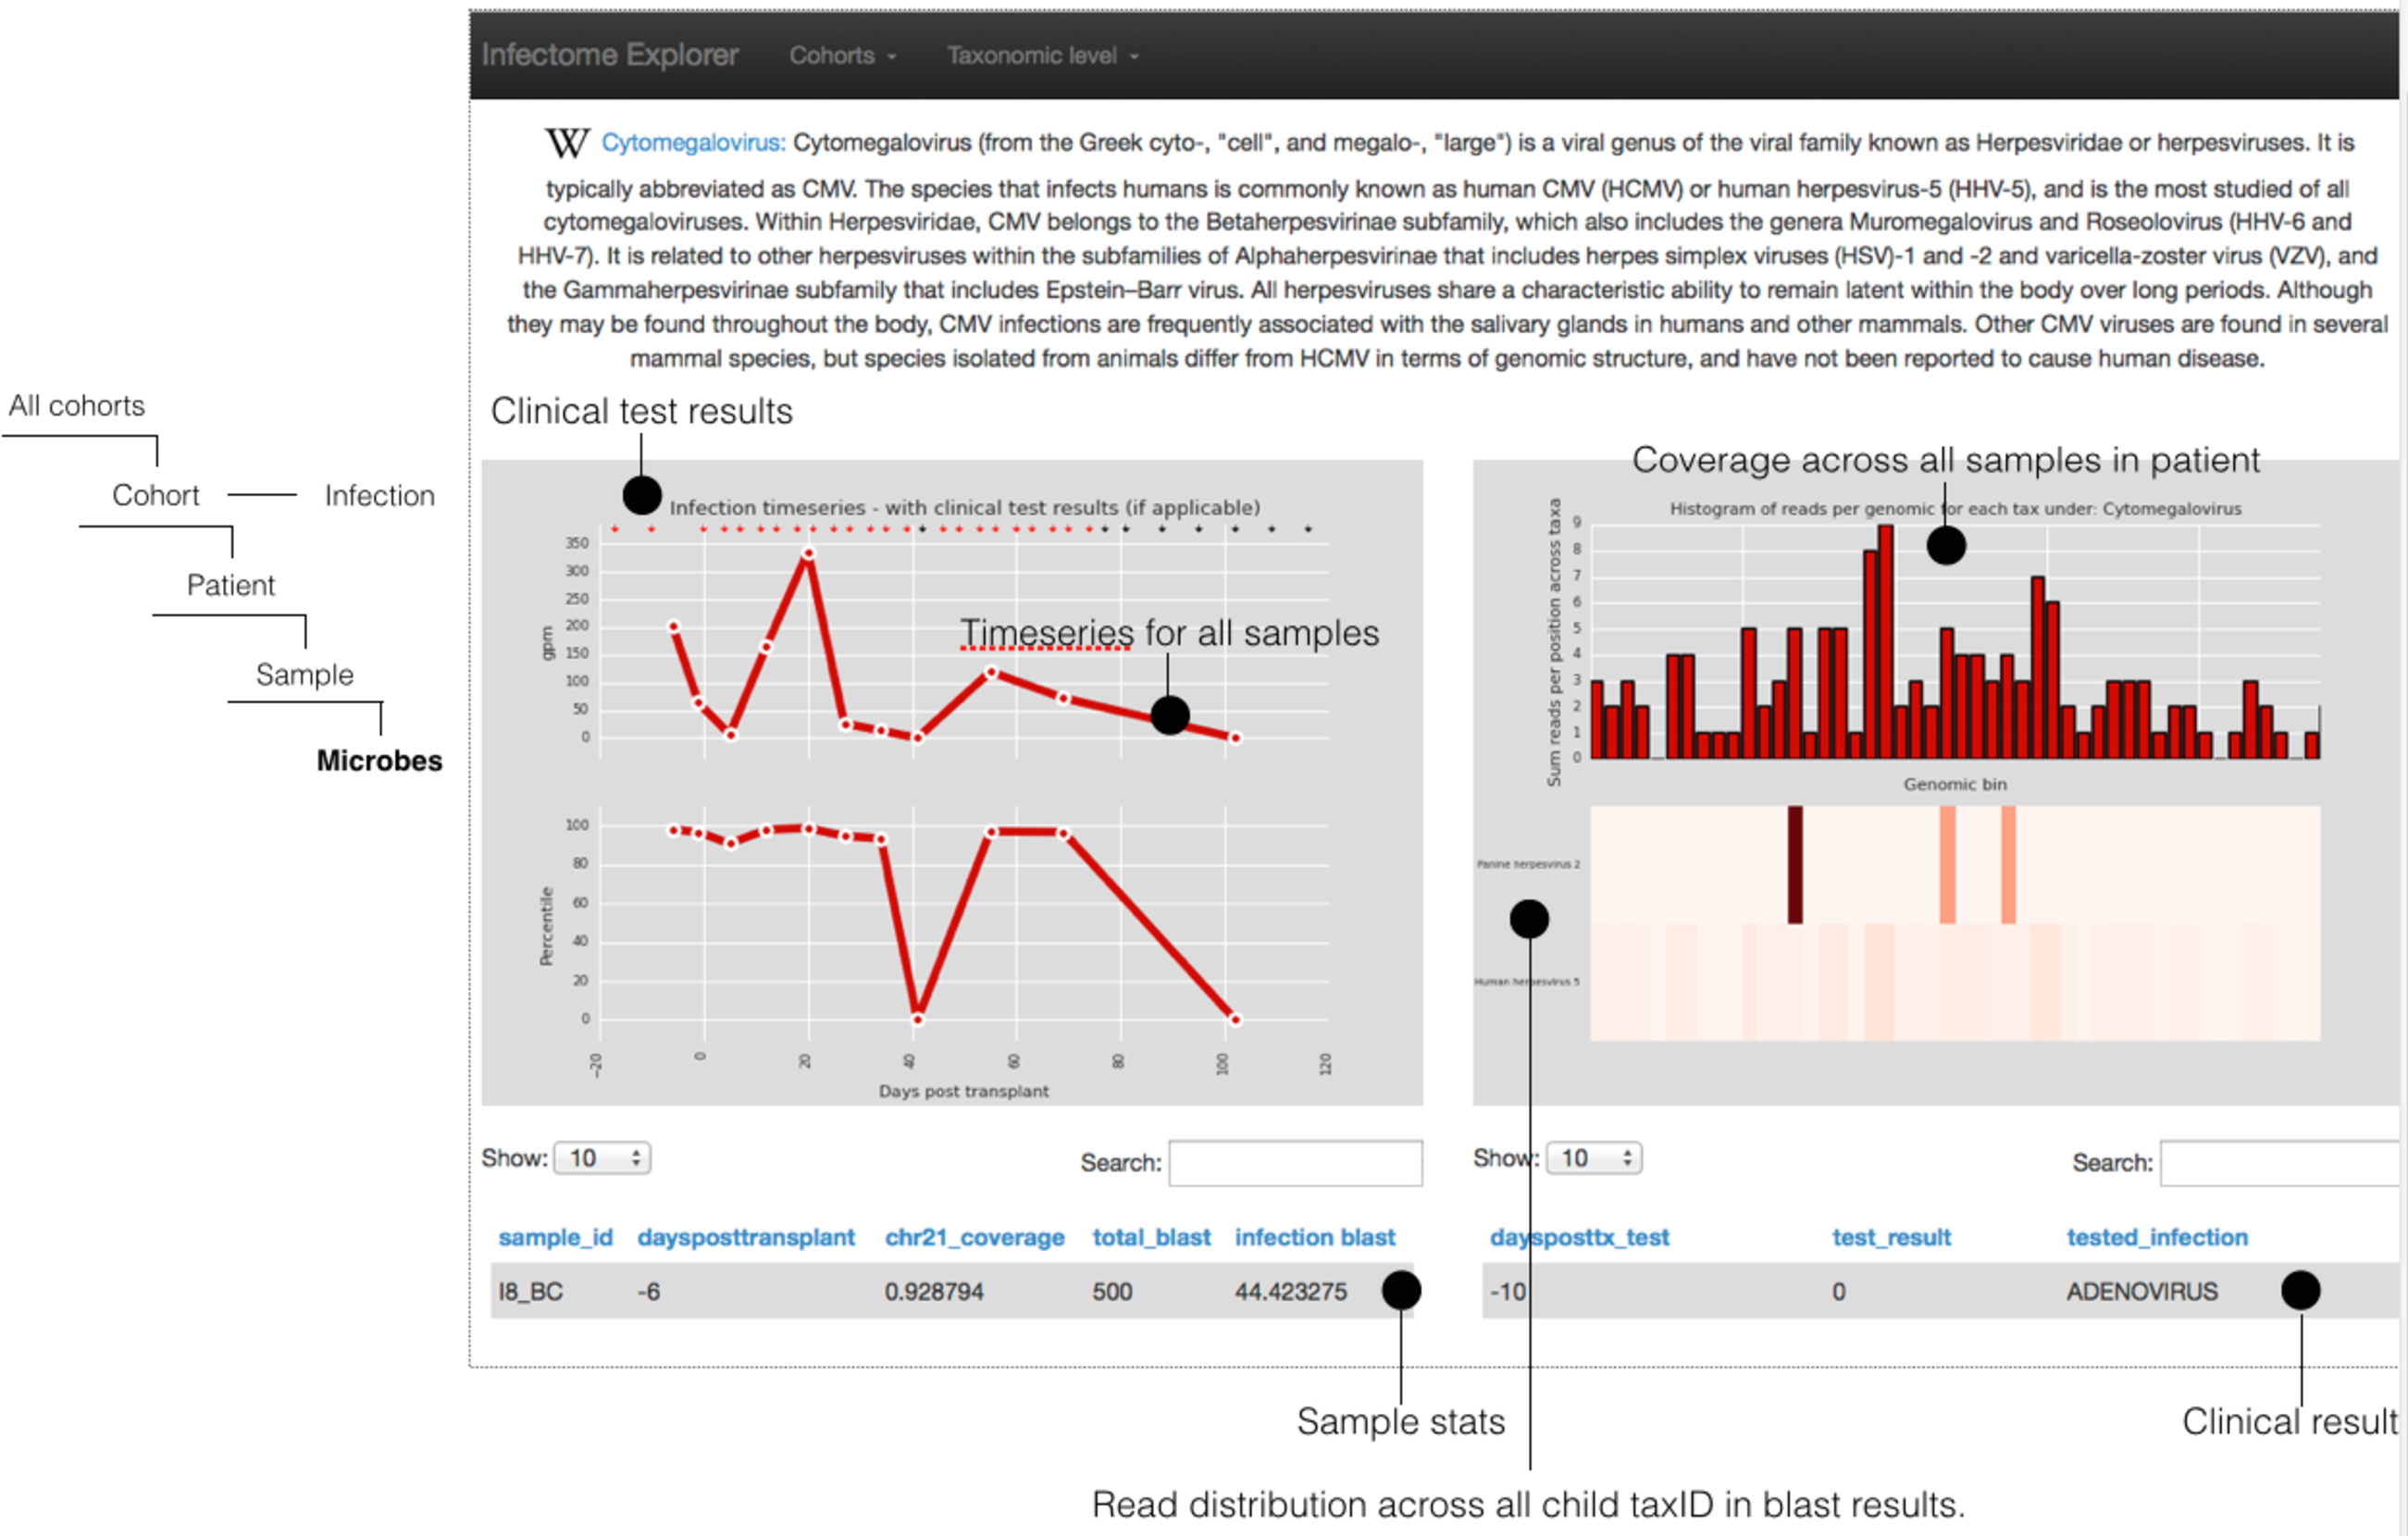
\includegraphics[width=150mm,scale=0.5]{Figures/Fig7}
\caption{Infectione timeseries and coverage}
\label{fig:Fig7}
\end{figure*}

To demonstrate clinical use of this application, we consider the case of I6, a pediatric bone marrow patient with severe respiratory complications. We collected longitudinal cell-free DNA samples across over the course of post-transplant therapy and processed the data with our application. From the application views, it was immediately clear that I6 a had very load of a rare Polyomavirus species, WU polyomavirus, that has been implicated in severe respiratory illnesses  Figure ~\ref{fig:Fig8}). Though the patient was tested for a similar polyomavirus, BK virus, those tests were negative. Indeed, the situation is similar to a scenario recently described in which NGS of cerebrospinal fluid identified an exotic pathogenic bacteria, leptospira, that explained severe hydrocephalus and status epilepticus \cite{Wilson:2014dv}. In this case, the patient died prior to clinical intervention based upon this information. However, the case does highlight the fact that unbiased and broad screening of potential pathogens in severe cases can reveal agents that escape conventional clinical testing and, in turn, will likely be a powerful supplement to existing clinical assays going forward.

\begin{figure*}
\center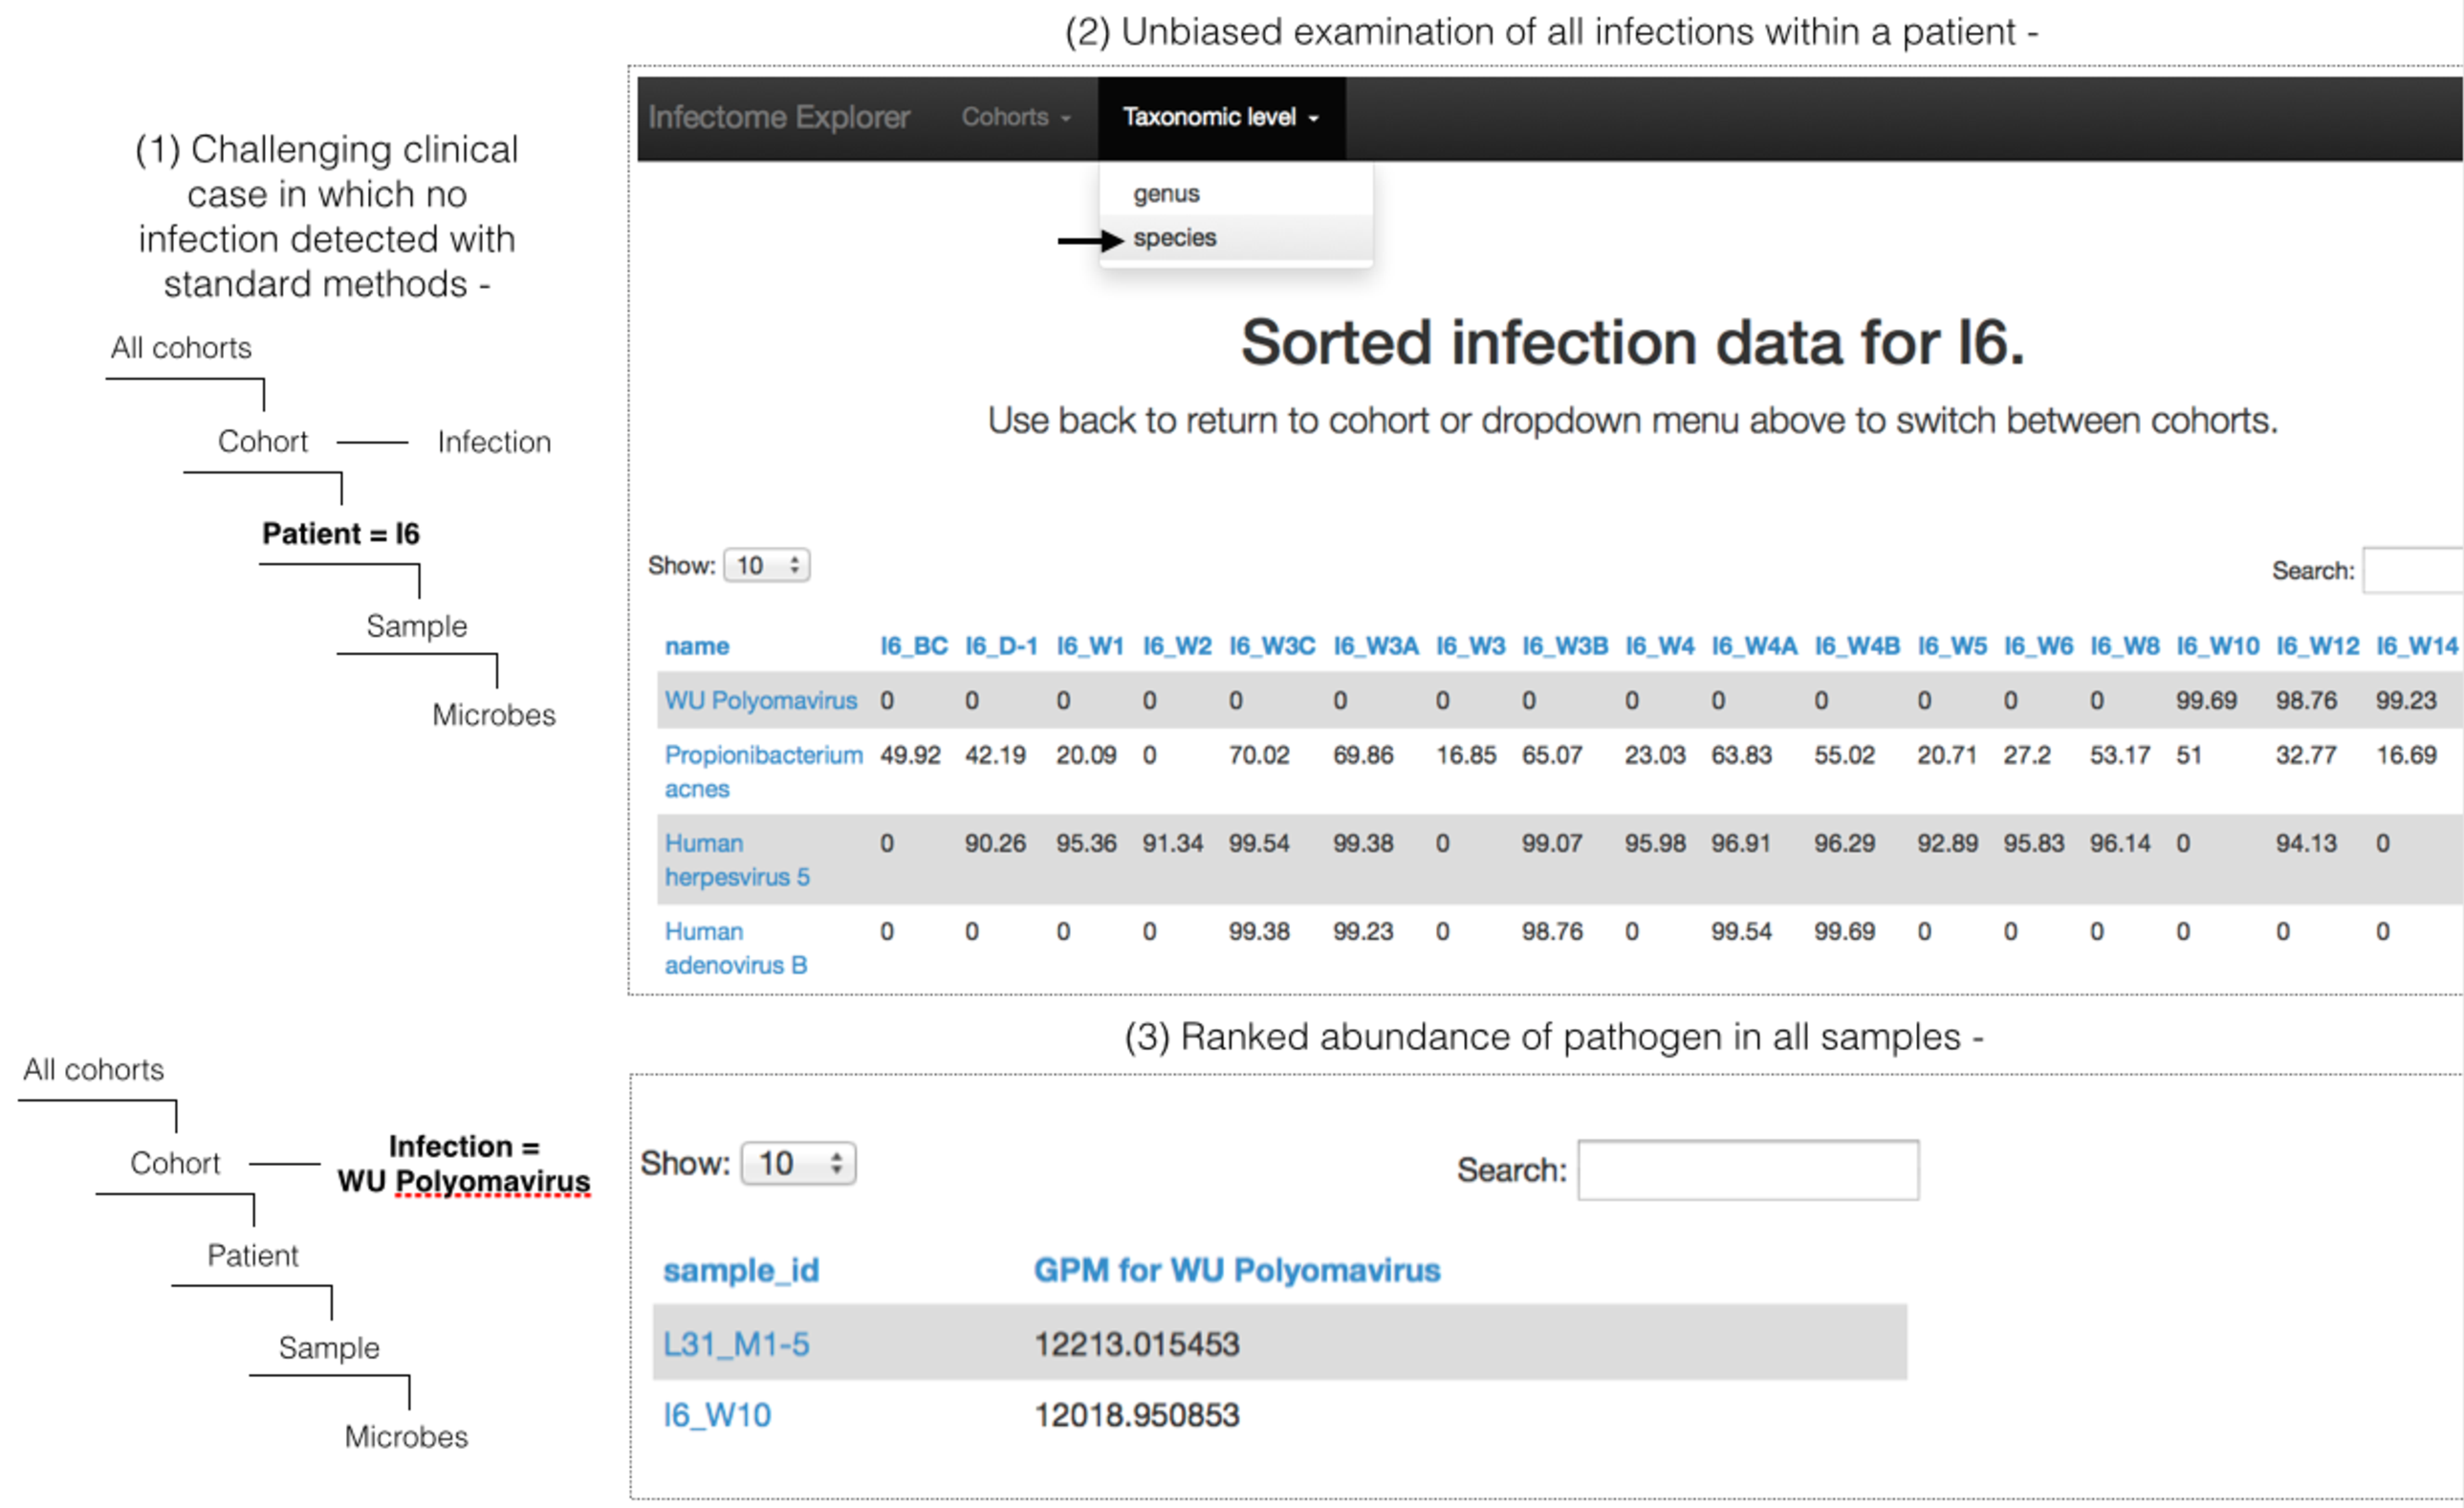
\includegraphics[width=150mm,scale=0.5]{Figures/Fig8}
\caption{Clinical use of infectome application}
\label{fig:Fig8}
\end{figure*}
